\newpage
\subsection{salsahView}
\subsubsection{gridView (search results and collections)}
\begin{figure}[!h]
    \centering
    \includegraphics[width=0.9\textwidth]{salsahView_grid.png}
    \caption{salsahView: grid (inspired by the old light table and the LFI news)}
\end{figure}

\subsubsection{listView (search results)}
\begin{figure}[!h]
    \centering
    \includegraphics[width=0.9\textwidth]{salsahView_list.png}
    \caption{salsahView: list (inspired by Google's inbox}
\end{figure}

\newpage

\subsubsection{tableView (search results of one resource type)}
\begin{figure}[!h]
    \centering
    \includegraphics[width=0.9\textwidth]{salsahView_table.png}
    \caption{salsahView: table (inspired by Excel)}
\end{figure}

From the list view (grid, list or tableView) the user can select more than one resource (well known from e-mail applications). In that case, an additional header provides some tools to do something with the selected resources. If the user selects some resources which are from the same resource type, he can edit them by one click. A modal box shows the properties of the selected resources. It's the same process as Apple's iTunes has (s. Fig. \ref{fig:itunes}).

\begin{figure}[!h]
    \centering
    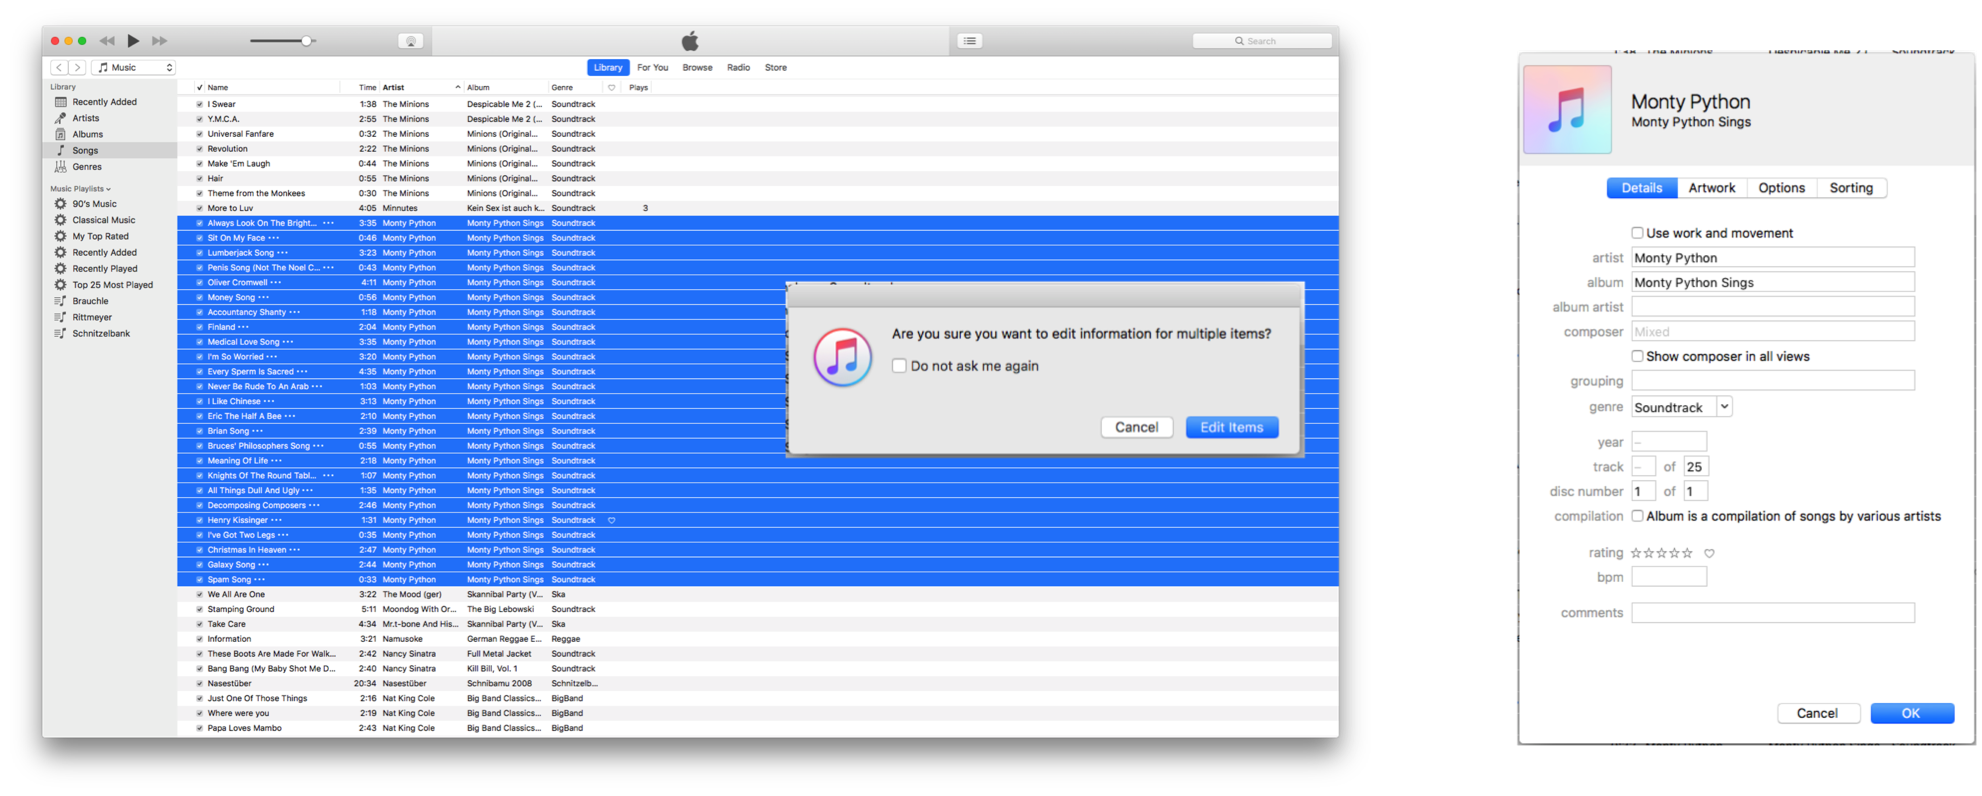
\includegraphics[width=0.9\textwidth]{iTunes-edit-selection.png}
    \caption{Example from iTunes: Selection of some songs; ``Get info'' opens a modal box, where the user can edit the properties for the whole selection.}
    \label{fig:itunes}
\end{figure}




\subsubsection{resourceView}
\begin{figure}[!h]
    \centering
    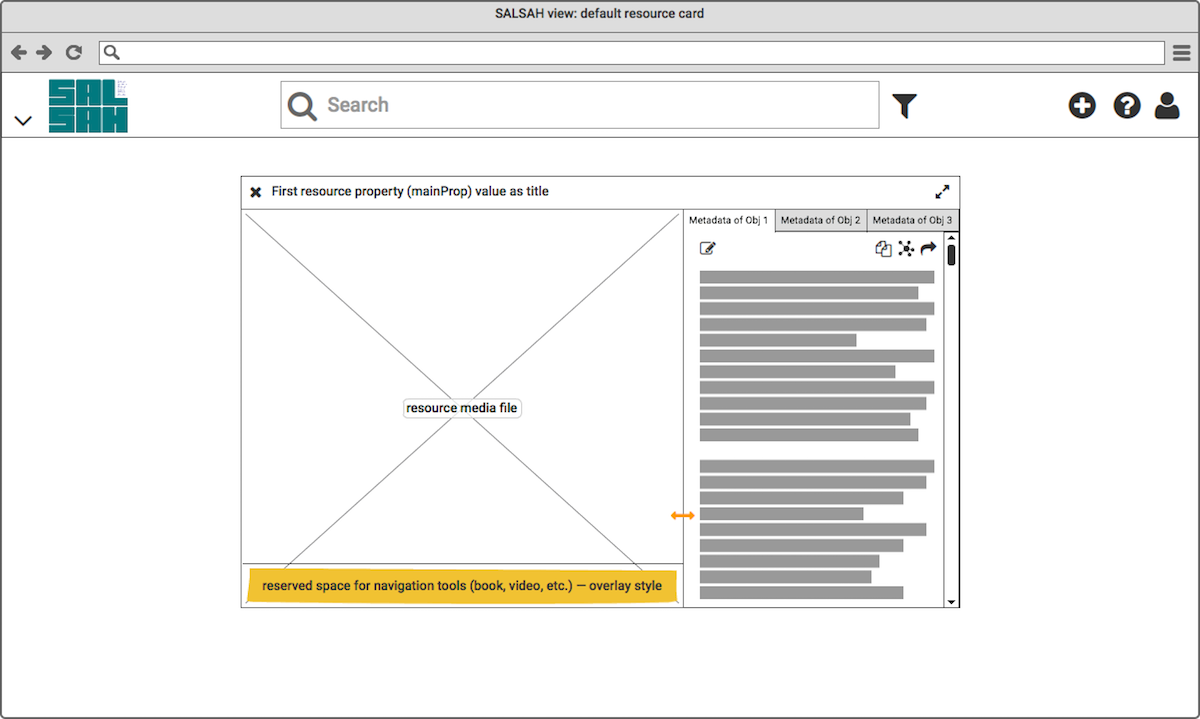
\includegraphics[width=0.9\textwidth]{salsahView_resource.png}
    \caption{salsahView: default resource card/modal (inspired by the window element of elementary OS)}
\end{figure}



\subsubsection{splitView (compare resources)}
Resource comparison viewer with a maximum of six flexible boxes.

\begin{figure}[!h]
    \centering
    \includegraphics[width=0.9\textwidth]{salsahView_split.png}
    \caption{salsahView: split (inspired by codepen.io)}
\end{figure}

\subsubsection{graphView}
Something with D3.js (d3js.org)

\subsubsection{dashboardView}
Place for activity thread includes updates from all projects the user is part of or has subscribed to. Activity thread should also be possible for user's activity.
